\label{chapter3}
\boldmath

\chapter{Data and Research Methodology}
\section{Introduction}
The data obtained and the procedures used for data gathering and analysis are the key topics of this chapter. It begins with description of the study area, which is comprised of Ghana's four agro-ecological zones. The study data, or information gathered, is then presented. Data analysis was also covered in this chapter.


\section{Study Area}
\begin{figure}[!ht]
	\centering
	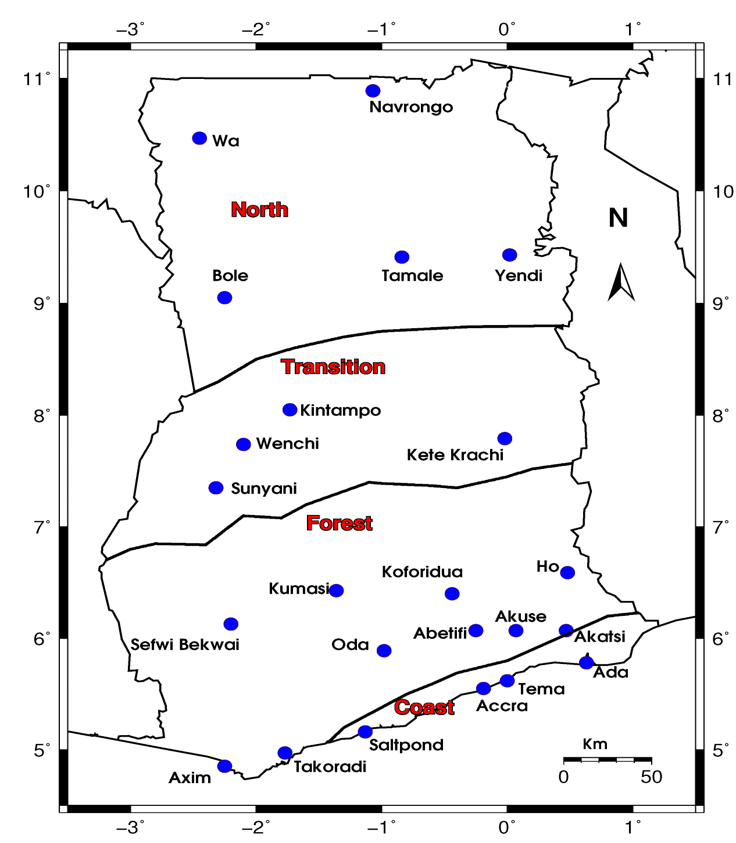
\includegraphics[scale=0.7]{project-picture.png}
	\caption{Map of Ghana showing the selected study areas. Adapted from \cite{amekudzi2015variabilities}}
	\label{fig.1}
\end{figure}

The Ghana's agro-ecological zones are the subject of this research. Fores, Northern, Transition,  and Coastal zones are the four agro-ecological zone.
Various cities make up each of these agro-ecological zones. We chose four cities across the various zones.\\

\noindent \textbf{Tamale} is the focus city for the Northern zone.It is the capital town of the northern region of Ghana. Tamale is the second-largest city in Ghana in terms of area. According to the 2012 census, the city has a population of 562,919 people. Located 600 kilometers (370 miles) north of Accra, the town is a popular tourist destination. It's location co-ordinate are latitude: $9^o$ 24' 2.84" N and longitude: $0^o$ 50' 21.48" E.\\

\noindent \textbf{Navrongo}  is a town in Upper East Region of Ghana, near the Burkina Faso border, and the capital of the Kassena-Nankana District. The capital of the Kassena-Nankana District, which is located in northern Ghana's Upper East Region, is Navrongo. In 2012, there were 27,306 people living in Navrongo. It's location co-ordinate are latitude: $10^o$ 53' 44" N and longitude: $1^o$ 05' 31" W.\\

\noindent \textbf{Kumasi} is the focus city for the Forest zone. Kumasi Metropolis is the capital of Ashanti and is located on the semi-island exclave Ashantiland in Ghana. Kumasi, the Ashanti capital city, is also known as Kumasi metropolis. Kumasi is located in a rain forest environment 30 kilometers north-east of Lake Bosumtwi, a crater lake. Kumasi is located west and south of Lake Volta, a massive artificial reservoir finished in 1965, and north of Crater Lake Lake Bosumtwi in Ashanti, some 500 kilometers north of the Equator and 200 kilometers (100 miles) north of the Gulf of Guinea. It's location co-ordinate are latitude: $6^o$ 41' 18.53" N and longitude: $-1^o$ 37' 27.95" W.\\

\noindent \textbf{Accra} is the focus city for the Coastal zone. It is Ghana's capital and largest city. It is also the coterminous capital of the Greater Accra Region and the Accra Metropolitan District. It's location co-ordinate are latitude: $5^o$ 33' 21.67" N and longitude: $0^o$ 11' 48.84" E.




\section{Data}
The Ghana Meteorological Agency (GMet) provided temperature data for the various agro-ecological zones. The data for temperature values spanned from the period of 1981–2020. These are the actual temperature values recorded at the various synoptic stations. The spatial and temporal resolution of the dataset are yearly and point data respectively.

\begin{table}[!ht]
	\begin{center}
		\caption{A table showing data used}
		\resizebox{\textwidth}{!}{
		\begin{tabular}{|l|l|l|l|l|}
			\hline
			DATA & SPATIAL RESOLUTION & TEMPORAL RESOLUTION & DURATION & SOURCE \\
			\hline
			Minimum Temperature & Point Data & Yearly & 1981-2020 & GMET \\
			\hline
			Maximum Temperature & Point Data & Yearly & 1981-2020 & GMET \\
			\hline
			Mean Temperature & Point Data & Yearly & 1981-2020 & GMET \\
			\hline
		\end{tabular}}
	\end{center}
	\label{tab:label}
\end{table}



\section{Analysis}
According to \cite{paaijmans2012warmer} the standard formulation for vectorial capacity (vc) is

 
\begin{equation}\label{vc}
	vc = {\dfrac{ma^{2}bcp^{Eip}}{-In(p)}}
\end{equation}

\noindent where vc is the vectorial capacity of the malaria vector,Eip is the extrinsic incubation period, p is the monthly vectorial survival and a, b, c and m are parameters explained below in tabular form with their respective values.


\begin{table}
\begin{center}
	\caption{A table showing parameter values used}
	\resizebox{\textwidth}{!}{
	\begin{tabular}{ |l| l | }
		\hline
		$PARAMETER$    & $VALUE$ \\
		\hline 
		Vector biting frequency, \textbf{a}    & $0.01-0.5 day^{-1}$ \\ 
		Probability of a person becoming infected, \textbf{b}    & $0.02-0.5$ \\
		Probability of a vector becoming infected, \textbf{c}  &    $0.5$\\ 
		Vector: Human ratio, \textbf{m}     & $0.5-4.0$ \\ 
		\hline	
	\end{tabular}}
\end{center}
\end{table}

\noindent Both the monthly vectorial survival, p and extrinsic incubation period, Eip depends on the temperature and these were calculated using \ref{p} and \ref{eip} respectively.\\

\noindent The daily vectorial survival, 

\begin{equation}\label{p}
	p = -0.00082T^2 + 0.0367T + 0.522
\end{equation}

\begin{center}
(source: \citep{lunde2013malaria})
\end{center}

\noindent where T represents the temperature.


\noindent Extrinsic incubation period, 
\begin{equation}\label{eip}
	Eip = {\dfrac{111}{T-16}}
\end{equation}

\begin{center}
	(source: \citep{detinova1962age}) 
\end{center}


\noindent where T represents the temperature. \\

 
\noindent The capacity of malaria vectors was then calculated using \ref{vc} after both the survival probability and the extrinsic incubation period were calculated using their respective functions specified above. This aid in achieving our objectives by determining the influence of seasonal  temperature  change on the survival and malaria transmission capacity of malaria vectors. Also to determine whether  the survival and vectorial capacity of malaria vectors differ as a function of climate and environment in Ghana.







